\documentclass[aspectratio=169]{beamer}

% ============================================================
% THEME AND PACKAGES
% ============================================================
\usetheme{metropolis}
\usepackage[utf8]{inputenc}
\usepackage[T1]{fontenc}
\usepackage[english]{babel}
\usepackage{graphicx}
\usepackage{booktabs}
\usepackage{xcolor}
\usepackage{tikz}
\usepackage{pgfplots}
\pgfplotsset{compat=1.18}
\usetikzlibrary{shapes,arrows,positioning,fit,backgrounds,calc,decorations.pathreplacing}
\usepackage{tcolorbox}
\tcbuselibrary{skins,breakable}
\usepackage{setspace}
\usepackage{microtype}
\usepackage{hyperref}

% ============================================================
% COLOR SCHEME
% ============================================================
\definecolor{primarydark}{RGB}{15,23,42}
\definecolor{primaryblue}{RGB}{30,64,175}
\definecolor{accentcyan}{RGB}{6,182,212}
\definecolor{accentorange}{RGB}{251,146,60}
\definecolor{accentred}{RGB}{239,68,68}
\definecolor{accentgreen}{RGB}{34,197,94}
\definecolor{accentpurple}{RGB}{168,85,247}
\definecolor{lightgray}{RGB}{241,245,249}
\definecolor{textgray}{RGB}{71,85,105}

\definecolor{chartcolor1}{RGB}{231,76,60}
\definecolor{chartcolor2}{RGB}{52,152,219}
\definecolor{chartcolor3}{RGB}{46,204,113}
\definecolor{chartcolor4}{RGB}{241,196,15}
\definecolor{chartcolor5}{RGB}{155,89,182}
\definecolor{chartcolor6}{RGB}{230,126,34}

% ============================================================
% BEAMER THEME CONFIGURATION
% ============================================================
\setbeamercolor{normal text}{fg=primarydark,bg=white}
\setbeamercolor{alerted text}{fg=accentred}
\setbeamercolor{example text}{fg=accentgreen}
\setbeamercolor{frametitle}{bg=primarydark,fg=white}
\setbeamercolor{title separator}{fg=accentcyan}
\setbeamercolor{progress bar}{fg=accentcyan,bg=primarydark!20}
\setbeamercolor{block title}{fg=white,bg=primaryblue}
\setbeamercolor{block body}{fg=primarydark,bg=lightgray}
\setbeamercolor{block title alerted}{fg=white,bg=accentred}
\setbeamercolor{block body alerted}{fg=primarydark,bg=accentred!8}
\setbeamercolor{block title example}{fg=white,bg=accentgreen!80!black}
\setbeamercolor{block body example}{bg=accentgreen!8}
\setbeamercolor{itemize item}{fg=primaryblue}
\setbeamercolor{enumerate item}{fg=primaryblue}

\metroset{
  titleformat=regular,
  sectionpage=progressbar,
  numbering=fraction,
  progressbar=frametitle,
  block=fill
}

% ============================================================
% CUSTOM BOXES
% ============================================================
\newtcolorbox{infobox}[1]{
  enhanced,
  colback=accentcyan!5,
  colframe=accentcyan,
  coltext=primarydark,
  title={\textbf{#1}},
  coltitle=white,
  colbacktitle=accentcyan,
  fonttitle=\sffamily\bfseries\small,
  fontupper=\sffamily\footnotesize,
  arc=3pt,
  boxrule=0pt,
  leftrule=3pt,
  toptitle=5pt,
  bottomtitle=5pt,
  left=8pt, right=8pt, top=4pt, bottom=6pt,
  before skip=6pt,
  after skip=6pt
}

\newtcolorbox{warnbox}[1]{
  enhanced,
  colback=accentorange!8,
  colframe=accentorange,
  coltext=primarydark,
  title={\textbf{#1}},
  coltitle=accentorange!80!black,
  colbacktitle=accentorange!25,
  fonttitle=\sffamily\bfseries\small,
  fontupper=\sffamily\footnotesize,
  arc=3pt,
  boxrule=0pt,
  leftrule=3pt,
  toptitle=5pt,
  bottomtitle=5pt,
  left=8pt, right=8pt, top=4pt, bottom=6pt,
  before skip=6pt,
  after skip=6pt
}

\newtcolorbox{dangerbox}[1]{
  enhanced,
  colback=accentred!5,
  colframe=accentred,
  coltext=primarydark,
  title={\textbf{#1}},
  coltitle=white,
  colbacktitle=accentred,
  fonttitle=\sffamily\bfseries\small,
  fontupper=\sffamily\footnotesize,
  arc=3pt,
  boxrule=0pt,
  leftrule=3pt,
  toptitle=5pt,
  bottomtitle=5pt,
  left=8pt, right=8pt, top=4pt, bottom=6pt,
  before skip=6pt,
  after skip=6pt
}

% ============================================================
% TYPOGRAPHY
% ============================================================
\setbeamerfont{title}{size=\LARGE,series=\bfseries}
\setbeamerfont{subtitle}{size=\normalsize}
\setbeamerfont{frametitle}{size=\large,series=\bfseries}
\setbeamerfont{block title}{size=\small,series=\bfseries}

\setlength{\leftmargini}{1em}
\setlength{\leftmarginii}{0.8em}

\newcommand{\code}[1]{\texttt{\textcolor{primaryblue}{#1}}}

% ============================================================
% TITLE PAGE
% ============================================================
\title{Ransomware}
\subtitle{A Comprehensive Overview of the Threat Landscape}
\date{\today}
\institute{IT Security -- Educational Presentation}

\begin{document}

% ============================================================
% TITLE SLIDE
% ============================================================
{
\setbeamertemplate{background}{
  \begin{tikzpicture}[overlay,remember picture]
    \shade[top color=primarydark,bottom color=primaryblue!50!primarydark]
      (current page.south west) rectangle (current page.north east);
    \draw[accentcyan,line width=2pt]
      ([yshift=-0.5cm]current page.center) ++(-5,0) -- ++(10,0);
  \end{tikzpicture}
}
\setbeamercolor{title}{fg=white}
\setbeamercolor{subtitle}{fg=accentcyan}
\setbeamercolor{institute}{fg=white!60}
\setbeamercolor{date}{fg=white!60}
\begin{frame}[plain]
  \vspace{2cm}
  \begin{center}
    {\usebeamerfont{title}\usebeamercolor[fg]{title}\inserttitle}\\[0.8em]
    {\usebeamerfont{subtitle}\usebeamercolor[fg]{subtitle}\insertsubtitle}\\[1.5em]
    {\footnotesize\usebeamercolor[fg]{institute}\insertinstitute}\\[0.3em]
    {\footnotesize\usebeamercolor[fg]{date}\insertdate}
  \end{center}
\end{frame}
}

% ============================================================
% AGENDA
% ============================================================
\begin{frame}{Agenda}
  \tableofcontents
\end{frame}

% ============================================================
% SECTION 1: WHAT IS RANSOMWARE?
% ============================================================
\section{What is Ransomware?}

\begin{frame}{Definition}
  \textbf{Ransomware} is a type of malicious software that restricts access to a computer system or its data -- typically through \alert{encryption} -- and demands a \alert{ransom payment} for restoration.

  \vspace{1em}

  \begin{columns}[T]
    \begin{column}{0.48\textwidth}
      \begin{block}{Core Characteristics}
        \begin{itemize}
          \item Denies access to files or systems
          \item Demands payment (cryptocurrency)
          \item Uses strong encryption algorithms
          \item Often includes a deadline/timer
        \end{itemize}
      \end{block}
    \end{column}
    \begin{column}{0.48\textwidth}
      \begin{block}{Typical Targets}
        \begin{itemize}
          \item Hospitals \& healthcare
          \item Government agencies
          \item Educational institutions
          \item Critical infrastructure
          \item Small/medium businesses
        \end{itemize}
      \end{block}
    \end{column}
  \end{columns}
\end{frame}

\begin{frame}{How Ransomware Works -- High-Level Overview}
  \centering
  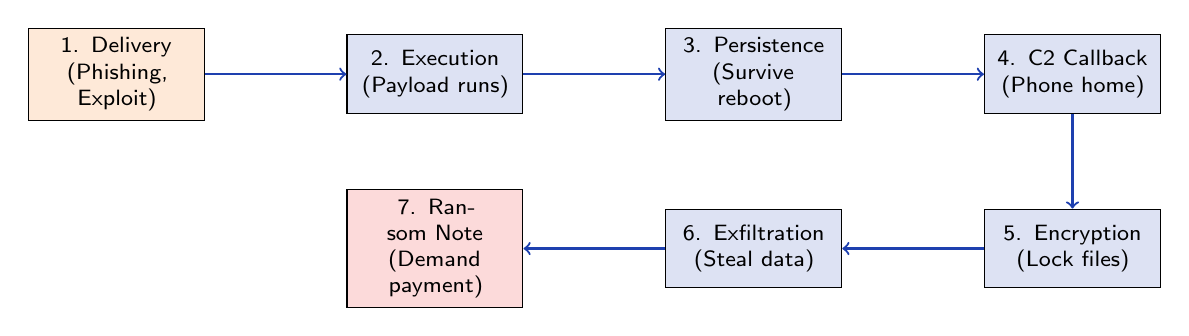
\begin{tikzpicture}[
    node distance=1.8cm,
    box/.style={rectangle, draw, fill=primaryblue!15, minimum width=2.2cm, minimum height=1cm, text width=2cm, align=center, font=\footnotesize\sffamily},
    arrow/.style={->, thick, primaryblue}
  ]
    \node[box, fill=accentorange!20] (delivery) {1. Delivery\\(Phishing, Exploit)};
    \node[box, right=of delivery] (exec) {2. Execution\\(Payload runs)};
    \node[box, right=of exec] (persist) {3. Persistence\\(Survive reboot)};
    \node[box, right=of persist] (c2) {4. C2 Callback\\(Phone home)};
    \node[box, below=1.2cm of c2] (encrypt) {5. Encryption\\(Lock files)};
    \node[box, left=of encrypt] (exfil) {6. Exfiltration\\(Steal data)};
    \node[box, left=of exfil, fill=accentred!20] (ransom) {7. Ransom Note\\(Demand payment)};

    \draw[arrow] (delivery) -- (exec);
    \draw[arrow] (exec) -- (persist);
    \draw[arrow] (persist) -- (c2);
    \draw[arrow] (c2) -- (encrypt);
    \draw[arrow] (encrypt) -- (exfil);
    \draw[arrow] (exfil) -- (ransom);
  \end{tikzpicture}
\end{frame}

% ============================================================
% SECTION 2: HISTORY AND EVOLUTION
% ============================================================
\section{History and Evolution}

\begin{frame}{The Origins: AIDS Trojan (1989)}
  \begin{columns}[T]
    \begin{column}{0.55\textwidth}
      \textbf{The first known ransomware:}
      \begin{itemize}
        \item Created by Dr.\ Joseph Popp
        \item Distributed via 20,000 floppy disks at a WHO conference
        \item Labeled ``AIDS Information -- Introductory Diskette''
        \item Encrypted file names on the C: drive after 90 reboots
        \item Demanded \$189 sent to a PO Box in Panama
        \item Used simple symmetric cryptography (easily reversible)
      \end{itemize}

      \vspace{0.5em}
      \begin{infobox}{Key Insight}
        Even in 1989, the fundamental concept was the same: deny access, demand payment. Only the delivery and crypto have evolved.
      \end{infobox}
    \end{column}
    \begin{column}{0.42\textwidth}
      \centering
      \begin{tikzpicture}[font=\sffamily\footnotesize]
        \node[rectangle, draw=primaryblue, fill=primaryblue!10, text width=4.5cm, align=center, rounded corners] {
          \textbf{AIDS Trojan (1989)}\\[0.3em]
          Floppy disk distribution\\
          Symmetric encryption\\
          \$189 ransom via mail\\[0.3em]
          \textit{Easily defeated}
        };
      \end{tikzpicture}
    \end{column}
  \end{columns}
\end{frame}

\begin{frame}{Evolution Timeline}
  \footnotesize
  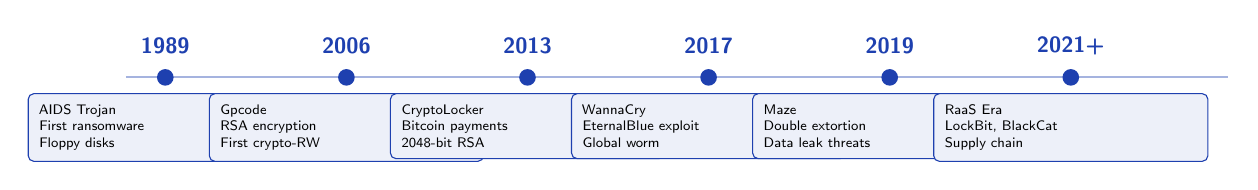
\begin{tikzpicture}[
    event/.style={rectangle, draw=primaryblue, fill=primaryblue!8, text width=3.2cm, align=left, font=\tiny\sffamily, rounded corners=2pt, inner sep=4pt},
    yearstyle/.style={font=\footnotesize\sffamily\bfseries, primaryblue},
    line/.style={thick, primaryblue!40}
  ]
    % Timeline line
    \draw[line] (0,0) -- (14,0);

    % Events
    \node[yearstyle] at (0.5, 0.4) {1989};
    \node[event, below] at (0.5, -0.2) {AIDS Trojan\\First ransomware\\Floppy disks};

    \node[yearstyle] at (2.8, 0.4) {2006};
    \node[event, below] at (2.8, -0.2) {Gpcode\\RSA encryption\\First crypto-RW};

    \node[yearstyle] at (5.1, 0.4) {2013};
    \node[event, below] at (5.1, -0.2) {CryptoLocker\\Bitcoin payments\\2048-bit RSA};

    \node[yearstyle] at (7.4, 0.4) {2017};
    \node[event, below] at (7.4, -0.2) {WannaCry\\EternalBlue exploit\\Global worm};

    \node[yearstyle] at (9.7, 0.4) {2019};
    \node[event, below] at (9.7, -0.2) {Maze\\Double extortion\\Data leak threats};

    \node[yearstyle] at (12.0, 0.4) {2021+};
    \node[event, below] at (12.0, -0.2) {RaaS Era\\LockBit, BlackCat\\Supply chain};

    % Dots on timeline
    \foreach \x in {0.5,2.8,5.1,7.4,9.7,12.0}
      \fill[primaryblue] (\x, 0) circle (3pt);
  \end{tikzpicture}

  \vspace{1em}
  \begin{center}
    \textbf{Key trend:} From hobbyist experiments $\rightarrow$ organized cybercrime $\rightarrow$ state-sponsored operations
  \end{center}
\end{frame}

\begin{frame}{Landmark Attacks}
  \begin{columns}[T]
    \begin{column}{0.48\textwidth}
      \begin{alertblock}{WannaCry (May 2017)}
        \footnotesize
        \begin{itemize}
          \item Exploited EternalBlue (NSA-leaked SMB vulnerability)
          \item Infected 230,000+ computers in 150 countries
          \item Hit NHS (UK), FedEx, Renault, Deutsche Bahn
          \item Caused \$4--8 billion in damages
          \item Accidentally stopped by a kill switch domain registration
          \item Attributed to North Korea (Lazarus Group)
        \end{itemize}
      \end{alertblock}
    \end{column}
    \begin{column}{0.48\textwidth}
      \begin{alertblock}{NotPetya (June 2017)}
        \footnotesize
        \begin{itemize}
          \item Disguised as ransomware, actually a wiper
          \item Distributed via Ukrainian tax software update (MeDoc)
          \item Spread globally via EternalBlue + credential harvesting
          \item Maersk: rebuilt entire IT (45,000 PCs, 4,000 servers)
          \item Total damages: \$10+ billion
          \item Attributed to Russian military (GRU)
        \end{itemize}
      \end{alertblock}
    \end{column}
  \end{columns}
\end{frame}

\begin{frame}{Colonial Pipeline (2021)}
  \begin{columns}[T]
    \begin{column}{0.55\textwidth}
      \textbf{The attack that changed policy:}
      \begin{itemize}
        \item DarkSide ransomware group attacked Colonial Pipeline
        \item Pipeline supplies 45\% of US East Coast fuel
        \item Shut down for 6 days (May 7--12, 2021)
        \item Caused fuel shortages, panic buying, price spikes
        \item Company paid \$4.4 million in Bitcoin
        \item FBI recovered \$2.3 million (63.7 BTC)
      \end{itemize}

      \vspace{0.5em}
      \begin{dangerbox}{Impact}
        Led to US Executive Order on Cybersecurity. Ransomware elevated to national security threat. DarkSide disbanded shortly after.
      \end{dangerbox}
    \end{column}
    \begin{column}{0.42\textwidth}
      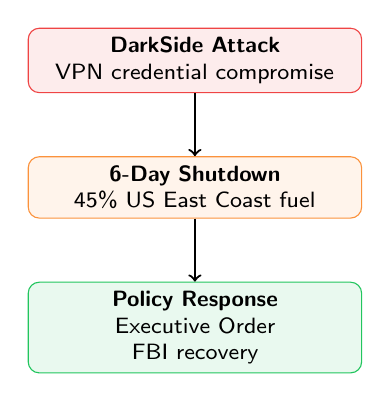
\begin{tikzpicture}[font=\sffamily\footnotesize, node distance=0.8cm]
        \node[rectangle, draw=accentred, fill=accentred!10, text width=4cm, align=center, rounded corners] (attack) {\textbf{DarkSide Attack}\\VPN credential compromise};
        \node[rectangle, draw=accentorange, fill=accentorange!10, text width=4cm, align=center, rounded corners, below=of attack] (impact) {\textbf{6-Day Shutdown}\\45\% US East Coast fuel};
        \node[rectangle, draw=accentgreen, fill=accentgreen!10, text width=4cm, align=center, rounded corners, below=of impact] (response) {\textbf{Policy Response}\\Executive Order\\FBI recovery};
        \draw[->, thick] (attack) -- (impact);
        \draw[->, thick] (impact) -- (response);
      \end{tikzpicture}
    \end{column}
  \end{columns}
\end{frame}

% ============================================================
% SECTION 3: TYPES OF RANSOMWARE
% ============================================================
\section{Types of Ransomware}

\begin{frame}{Fundamental Classification}
  \begin{columns}[T]
    \begin{column}{0.48\textwidth}
      \begin{block}{1. Crypto-Ransomware}
        \small
        \begin{itemize}
          \item \textbf{Encrypts} user files (documents, images, databases)
          \item System remains functional
          \item Uses strong encryption (AES, RSA, ChaCha20)
          \item Recovery without key is practically impossible
          \item \textbf{Examples:} CryptoLocker, LockBit, BlackCat
        \end{itemize}
      \end{block}
    \end{column}
    \begin{column}{0.48\textwidth}
      \begin{block}{2. Locker-Ransomware}
        \small
        \begin{itemize}
          \item \textbf{Locks} the entire system (screen lock)
          \item Files themselves are \textit{not} encrypted
          \item Often impersonates law enforcement (``FBI virus'')
          \item Easier to remove (boot from USB, safe mode)
          \item \textbf{Examples:} WinLocker, Police Ransomware
        \end{itemize}
      \end{block}
    \end{column}
  \end{columns}

  \vspace{0.8em}
  \begin{center}
    \textcolor{textgray}{\footnotesize Today, \textbf{crypto-ransomware} dominates ($>$95\% of incidents). Locker variants are largely obsolete.}
  \end{center}
\end{frame}

\begin{frame}{Modern Variants and Tactics}
  \begin{columns}[T]
    \begin{column}{0.48\textwidth}
      \begin{block}{3. Wipers (Destructive)}
        \footnotesize
        \begin{itemize}
          \item Disguised as ransomware but data is irrecoverable
          \item Goal: destruction, not profit
          \item Often state-sponsored (NotPetya, WhisperGate)
          \item No functional decryption mechanism exists
        \end{itemize}
      \end{block}
      \vspace{0.3em}
      \begin{block}{4. Leakware / Doxware}
        \footnotesize
        \begin{itemize}
          \item Threatens to \textbf{publish} stolen data
          \item Even if backups exist, victim still pressured
          \item Regulatory fines (GDPR) add leverage
          \item Data is often sold on darknet regardless
        \end{itemize}
      \end{block}
    \end{column}
    \begin{column}{0.48\textwidth}
      \begin{block}{5. RaaS (Ransomware-as-a-Service)}
        \footnotesize
        \begin{itemize}
          \item Subscription-based model for affiliates
          \item Provider handles malware development, C2 infra, negotiation
          \item Affiliate handles initial access and deployment
          \item Revenue split: typically 70/30 or 80/20
          \item Lowered barrier to entry massively
        \end{itemize}
      \end{block}
      \vspace{0.3em}
      \begin{block}{6. Intermittent Encryption}
        \footnotesize
        \begin{itemize}
          \item Only encrypts parts of each file (e.g., every other block)
          \item Files still unusable but encryption is 5--10x faster
          \item Harder for EDR to detect (fewer I/O anomalies)
          \item Used by LockFile, BlackCat, Play
        \end{itemize}
      \end{block}
    \end{column}
  \end{columns}
\end{frame}

% ============================================================
% SECTION 4: EXTORTION MODELS
% ============================================================
\section{Extortion Models}

\begin{frame}{The Evolution of Extortion}
  \centering
  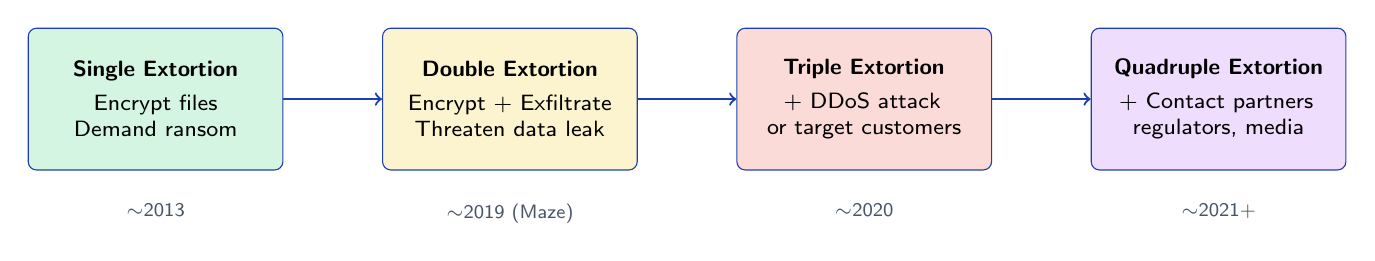
\begin{tikzpicture}[
    box/.style={rectangle, draw=primaryblue, fill=primaryblue!10, text width=3cm, align=center, font=\footnotesize\sffamily, rounded corners=3pt, minimum height=1.8cm},
    arrow/.style={->, thick, primaryblue},
    label/.style={font=\scriptsize\sffamily, text=textgray}
  ]
    \node[box, fill=chartcolor3!20] (single) at (0,0) {\textbf{Single Extortion}\\[0.3em]Encrypt files\\Demand ransom};
    \node[box, fill=chartcolor4!20] (double) at (4.5,0) {\textbf{Double Extortion}\\[0.3em]Encrypt + Exfiltrate\\Threaten data leak};
    \node[box, fill=chartcolor1!20] (triple) at (9,0) {\textbf{Triple Extortion}\\[0.3em]+ DDoS attack\\or target customers};
    \node[box, fill=accentpurple!20] (quadruple) at (13.5,0) {\textbf{Quadruple Extortion}\\[0.3em]+ Contact partners\\regulators, media};

    \draw[arrow] (single) -- (double);
    \draw[arrow] (double) -- (triple);
    \draw[arrow] (triple) -- (quadruple);

    \node[label, below=0.3cm of single] {$\sim$2013};
    \node[label, below=0.3cm of double] {$\sim$2019 (Maze)};
    \node[label, below=0.3cm of triple] {$\sim$2020};
    \node[label, below=0.3cm of quadruple] {$\sim$2021+};
  \end{tikzpicture}

  \vspace{1em}
  \begin{warnbox}{Key Trend}
    Even organizations with perfect backups can be extorted. Data theft and reputational damage create pressure independent of encryption.
  \end{warnbox}
\end{frame}

\begin{frame}{Double Extortion in Detail}
  \begin{columns}[T]
    \begin{column}{0.55\textwidth}
      \textbf{Pioneered by Maze (Nov 2019):}
      \begin{enumerate}
        \item Attacker gains initial access
        \item \textbf{Exfiltrate} sensitive data to attacker-controlled servers
        \item \textbf{Encrypt} files on victim network
        \item Demand ransom for decryption key
        \item If victim refuses: publish stolen data on \textbf{leak site}
      \end{enumerate}

      \vspace{0.5em}
      \textbf{Why this is devastating:}
      \begin{itemize}
        \item Backups don't help against data leaks
        \item GDPR fines can exceed ransom amount
        \item Competitive intelligence exposure
        \item Customer trust is permanently damaged
      \end{itemize}
    \end{column}
    \begin{column}{0.42\textwidth}
      \centering
      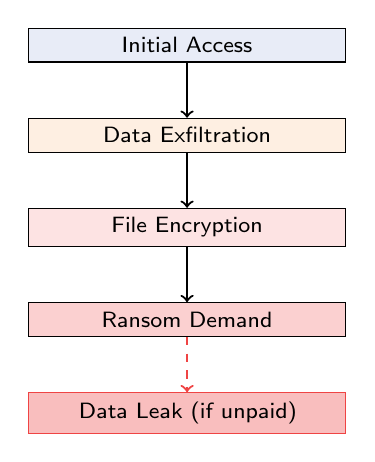
\begin{tikzpicture}[font=\sffamily\footnotesize, node distance=0.7cm]
        \node[rectangle, draw, fill=primaryblue!10, text width=3.8cm, align=center] (access) {Initial Access};
        \node[rectangle, draw, fill=accentorange!15, text width=3.8cm, align=center, below=of access] (exfil) {Data Exfiltration};
        \node[rectangle, draw, fill=accentred!15, text width=3.8cm, align=center, below=of exfil] (encrypt) {File Encryption};
        \node[rectangle, draw, fill=accentred!25, text width=3.8cm, align=center, below=of encrypt] (demand) {Ransom Demand};
        \node[rectangle, draw=accentred, fill=accentred!35, text width=3.8cm, align=center, below=of demand] (leak) {Data Leak (if unpaid)};

        \draw[->, thick] (access) -- (exfil);
        \draw[->, thick] (exfil) -- (encrypt);
        \draw[->, thick] (encrypt) -- (demand);
        \draw[->, thick, dashed, accentred] (demand) -- (leak);
      \end{tikzpicture}
    \end{column}
  \end{columns}
\end{frame}

% ============================================================
% SECTION 5: THE RANSOMWARE ECONOMY
% ============================================================
\section{The Ransomware Economy}

\begin{frame}{Ransomware-as-a-Service (RaaS)}
  \textbf{RaaS} transforms ransomware from individual attacks into a \alert{professional shadow economy}:

  \vspace{0.5em}
  \begin{columns}[T]
    \begin{column}{0.32\textwidth}
      \begin{block}{Initial Access Brokers}
        \footnotesize
        Specialists who sell network access to victim organizations. Methods:
        \begin{itemize}
          \item Phishing campaigns
          \item Exploit kits
          \item Stolen VPN credentials
          \item Insider recruitment
        \end{itemize}
        \textbf{Price:} \$500--\$100,000+
      \end{block}
    \end{column}
    \begin{column}{0.32\textwidth}
      \begin{block}{RaaS Operators}
        \footnotesize
        Develop and maintain the malware platform:
        \begin{itemize}
          \item Ransomware binary
          \item C2 infrastructure
          \item Negotiation portals
          \item Leak sites
          \item 24/7 ``support''
        \end{itemize}
        \textbf{Cut:} 20--30\% of ransom
      \end{block}
    \end{column}
    \begin{column}{0.32\textwidth}
      \begin{block}{Affiliates}
        \footnotesize
        The operators who execute attacks:
        \begin{itemize}
          \item Buy access
          \item Deploy ransomware
          \item Handle negotiation
          \item Collect payment
          \item Vary in skill level
        \end{itemize}
        \textbf{Cut:} 70--80\% of ransom
      \end{block}
    \end{column}
  \end{columns}
\end{frame}

\begin{frame}{Financial Impact -- Global Scale}
  \begin{columns}[T]
    \begin{column}{0.38\textwidth}
      \textbf{Estimated Global Damages}
      \vspace{0.5em}

      \begin{tabular}{ll}
        2017: & \textbf{\$5B}\\
        2019: & \textbf{\$11.5B}\\
        2021: & \textbf{\$20B}\\
        2024: & \textbf{\$42B}\\
        2031: & \textbf{\$265B} (est.)\\
      \end{tabular}

      \vspace{0.8em}
      \textcolor{accentred}{\textbf{+740\%}} increase in 7 years

      \vspace{0.5em}
      \footnotesize
      Average ransom payment in 2024: \textbf{\$2.73 million} (Sophos)

      \vspace{0.3em}
      Average downtime: \textbf{24 days}
    \end{column}
    \begin{column}{0.58\textwidth}
      \begin{tikzpicture}
        \begin{axis}[
          width=\textwidth,
          height=0.65\textheight,
          xlabel={\footnotesize Year},
          ylabel={\footnotesize Damages (Billion USD)},
          ymin=0, ymax=50,
          xtick={2015,2017,2019,2021,2024},
          ytick={0,10,20,30,40,50},
          grid=both,
          grid style={line width=.1pt, draw=lightgray},
          x tick label style={/pgf/number format/1000 sep={},font=\scriptsize},
          y tick label style={font=\scriptsize},
        ]
        \addplot[fill=chartcolor1!30,draw=chartcolor1,line width=1.5pt,mark=*,mark options={fill=chartcolor1,scale=0.8}] coordinates {
          (2015,0.325)(2017,5)(2019,11.5)(2021,20)(2024,42)
        } \closedcycle;
        \end{axis}
      \end{tikzpicture}
    \end{column}
  \end{columns}
\end{frame}

\begin{frame}{Professionalization: LockBit Case Study}
  \textbf{LockBit} exemplifies the professionalization of ransomware operations:

  \vspace{0.5em}
  \begin{columns}[T]
    \begin{column}{0.48\textwidth}
      \begin{block}{Business Features}
        \footnotesize
        \begin{itemize}
          \item Affiliate portal with dashboard
          \item Bug bounty program for their malware
          \item ``StealBit'' custom exfiltration tool
          \item Automatic negotiation via Tor
          \item Multiple encryption modes (fast, full, intermittent)
          \item Multi-OS support (Windows, Linux, VMware ESXi)
        \end{itemize}
      \end{block}
    \end{column}
    \begin{column}{0.48\textwidth}
      \begin{infobox}{LockBit Bug Bounty}
        ``Locker Bugs: Any errors during encryption \ldots\ that lead to corrupted files or to the possibility of decrypting files without getting a decryptor.''

        \vspace{0.3em}
        Rewards range from \$1,000 to \$1,000,000 for vulnerabilities in their infrastructure.
      \end{infobox}

      \vspace{0.3em}
      \begin{warnbox}{Takedown: Feb 2024}
        Operation Cronos (FBI + NCA + Europol) seized LockBit infrastructure. Group attempted comeback but lost affiliate trust.
      \end{warnbox}
    \end{column}
  \end{columns}
\end{frame}

\begin{frame}{ENISA Threat Landscape 2024}
  \begin{columns}[T]
    \begin{column}{0.35\textwidth}
      \textbf{Top EU Cyber Threats:}
      \begin{enumerate}
        \item DDoS/RDoS (46.31\%)
        \item \alert{Ransomware (27.33\%)}
        \item Data Breaches (15.87\%)
        \item Social Engineering (5.37\%)
        \item Malware (2.45\%)
        \item Zero-Day (0.11\%)
      \end{enumerate}

      \vspace{0.5em}
      \small\textbf{Ransomware: 2nd largest threat in Europe}

      \vspace{0.3em}
      \footnotesize
      Source: ENISA Threat Landscape Report 2024
    \end{column}
    \begin{column}{0.62\textwidth}
      \begin{tikzpicture}
        \begin{axis}[
          width=\textwidth,
          height=0.65\textheight,
          xbar,
          xlabel={\footnotesize Incidents (Thousands)},
          symbolic y coords={Zero-Day, Malware, Social Eng., Data, Ransomware, DDoS},
          ytick=data,
          nodes near coords,
          nodes near coords style={font=\scriptsize},
          xmin=0, xmax=2.8,
          bar width=0.4cm,
          y tick label style={font=\scriptsize},
          x tick label style={font=\scriptsize},
          enlarge y limits=0.12,
        ]
        \addplot[fill=chartcolor1,draw=chartcolor1!80!black] coordinates {
          (0.01,Zero-Day)(0.13,Malware)(0.29,Social Eng.)(0.84,Data)(1.45,Ransomware)(2.46,DDoS)
        };
        \end{axis}
      \end{tikzpicture}
    \end{column}
  \end{columns}
\end{frame}

% ============================================================
% SECTION 6: ATTACK LIFECYCLE
% ============================================================
\section{Attack Lifecycle (Cyber Kill Chain)}

\begin{frame}{The Ransomware Kill Chain}
  \centering
  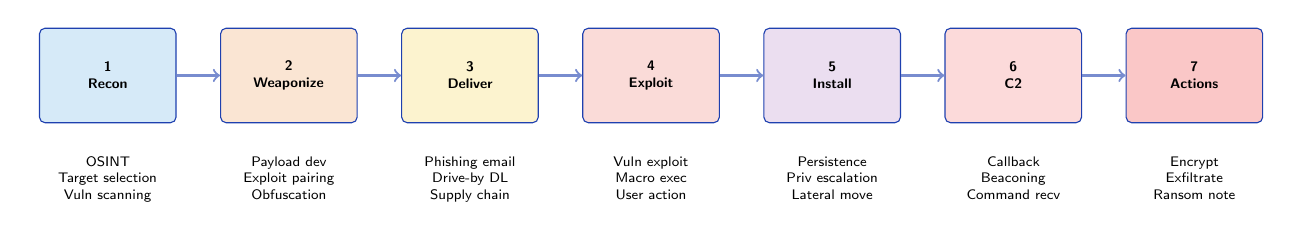
\begin{tikzpicture}[
    phase/.style args={#1}{
      rectangle,
      draw=primaryblue,
      fill=#1,
      minimum width=1.6cm,
      minimum height=1.2cm,
      text width=1.5cm,
      align=center,
      font=\tiny\sffamily\bfseries,
      rounded corners=2pt
    },
    desc/.style={font=\tiny\sffamily, text width=1.8cm, align=center},
    arrow/.style={->, thick, primaryblue!60}
  ]
    \node[phase=chartcolor2!20] (recon) at (0,0) {1\\Recon};
    \node[phase=chartcolor6!20] (weapon) at (2.3,0) {2\\Weaponize};
    \node[phase=chartcolor4!20] (deliver) at (4.6,0) {3\\Deliver};
    \node[phase=chartcolor1!20] (exploit) at (6.9,0) {4\\Exploit};
    \node[phase=chartcolor5!20] (install) at (9.2,0) {5\\Install};
    \node[phase=accentred!20] (c2) at (11.5,0) {6\\C2};
    \node[phase=accentred!30] (action) at (13.8,0) {7\\Actions};

    \node[desc, below=0.3cm of recon] {OSINT\\Target selection\\Vuln scanning};
    \node[desc, below=0.3cm of weapon] {Payload dev\\Exploit pairing\\Obfuscation};
    \node[desc, below=0.3cm of deliver] {Phishing email\\Drive-by DL\\Supply chain};
    \node[desc, below=0.3cm of exploit] {Vuln exploit\\Macro exec\\User action};
    \node[desc, below=0.3cm of install] {Persistence\\Priv escalation\\Lateral move};
    \node[desc, below=0.3cm of c2] {Callback\\Beaconing\\Command recv};
    \node[desc, below=0.3cm of action] {Encrypt\\Exfiltrate\\Ransom note};

    \draw[arrow] (recon) -- (weapon);
    \draw[arrow] (weapon) -- (deliver);
    \draw[arrow] (deliver) -- (exploit);
    \draw[arrow] (exploit) -- (install);
    \draw[arrow] (install) -- (c2);
    \draw[arrow] (c2) -- (action);
  \end{tikzpicture}

  \vspace{0.8em}
  \begin{infobox}{Dwell Time}
    Average time from initial access to encryption deployment: \textbf{5 days} (Mandiant M-Trends 2024). This window is critical for detection.
  \end{infobox}
\end{frame}

\begin{frame}{Phase 1: Initial Access}
  \textbf{How attackers get in:}

  \vspace{0.5em}
  \begin{columns}[T]
    \begin{column}{0.48\textwidth}
      \begin{block}{Phishing (Most Common)}
        \footnotesize
        \begin{itemize}
          \item Spear-phishing with malicious attachments
          \item Embedded macros in Office documents
          \item PDF files with JavaScript payloads
          \item Links to credential harvesting sites
          \item QR code phishing (quishing)
        \end{itemize}
      \end{block}
      \vspace{0.3em}
      \begin{block}{Exploiting Vulnerabilities}
        \footnotesize
        \begin{itemize}
          \item Unpatched VPN gateways (Fortinet, Pulse Secure)
          \item Remote Desktop Protocol (RDP) brute-force
          \item Exchange server exploits (ProxyShell)
          \item Log4Shell, MOVEit, Citrix Bleed
        \end{itemize}
      \end{block}
    \end{column}
    \begin{column}{0.48\textwidth}
      \begin{block}{Drive-by Downloads}
        \footnotesize
        \begin{itemize}
          \item Compromised legitimate websites
          \item Malicious ads (malvertising)
          \item Exploit kits (e.g., RIG, Magnitude)
          \item OS/browser detection for targeted payloads
        \end{itemize}
      \end{block}
      \vspace{0.3em}
      \begin{block}{Supply Chain \& Other}
        \footnotesize
        \begin{itemize}
          \item Compromised software updates (SolarWinds, Kaseya)
          \item MSP compromise (managed service providers)
          \item Stolen credentials from data breaches
          \item Insider threats / social engineering
        \end{itemize}
      \end{block}
    \end{column}
  \end{columns}
\end{frame}

\begin{frame}{Phase 2: Execution and Evasion}
  \begin{columns}[T]
    \begin{column}{0.48\textwidth}
      \textbf{Execution Techniques:}
      \begin{itemize}
        \item PowerShell / cmd scripts
        \item DLL side-loading
        \item Process injection (process hollowing)
        \item Living-off-the-land binaries (LOLBins)
        \item Reflective DLL loading
      \end{itemize}

      \vspace{0.5em}
      \textbf{Sandbox/VM Detection:}
      \begin{itemize}
        \item Check RAM $<$ 2--4 GB
        \item Check CPU cores $<$ 2
        \item Check disk size $<$ 60 GB
        \item Detect analysis tools (Wireshark, Procmon)
        \item Mouse movement detection
        \item Sleep acceleration detection
      \end{itemize}
    \end{column}
    \begin{column}{0.48\textwidth}
      \textbf{Evasion Techniques:}
      \begin{itemize}
        \item \textbf{Obfuscation:} String encryption, control flow flattening
        \item \textbf{Packing:} UPX, custom packers, crypters
        \item \textbf{AMSI Bypass:} Patching in-memory
        \item \textbf{EDR Evasion:} Direct syscalls, unhooking
        \item \textbf{Timestomping:} Modify file timestamps
        \item \textbf{Fileless:} Run entirely in memory
      \end{itemize}

      \vspace{0.5em}
      \begin{warnbox}{Rust \& Go Trend}
        Modern ransomware increasingly uses Rust or Go instead of C/C++, making reverse engineering harder due to complex binaries.
      \end{warnbox}
    \end{column}
  \end{columns}
\end{frame}

\begin{frame}{Phase 3: Persistence and Lateral Movement}
  \begin{columns}[T]
    \begin{column}{0.48\textwidth}
      \textbf{Persistence Mechanisms:}
      \begin{block}{Windows}
        \footnotesize
        \begin{itemize}
          \item Registry Run keys (\code{HKCU/HKLM})
          \item Scheduled Tasks (\code{schtasks})
          \item WMI Event Subscriptions
          \item DLL search order hijacking
          \item Boot/Logon scripts (GPO)
        \end{itemize}
      \end{block}
      \begin{block}{Linux}
        \footnotesize
        \begin{itemize}
          \item Systemd user services
          \item Cron jobs (\code{@reboot})
          \item \code{.bashrc} / \code{.profile} modification
          \item init.d scripts
        \end{itemize}
      \end{block}
    \end{column}
    \begin{column}{0.48\textwidth}
      \textbf{Lateral Movement:}
      \begin{block}{Techniques}
        \footnotesize
        \begin{itemize}
          \item \textbf{Credential Harvesting:} Mimikatz, LSASS dump
          \item \textbf{Pass-the-Hash:} Reuse NTLM hashes
          \item \textbf{RDP pivoting:} Jump between hosts
          \item \textbf{PsExec / WMI:} Remote execution
          \item \textbf{SMB shares:} Network drive encryption
          \item \textbf{AD exploitation:} DCSync, Kerberoasting
        \end{itemize}
      \end{block}

      \vspace{0.3em}
      \begin{infobox}{MITRE ATT\&CK}
        Ransomware typically maps to 40+ techniques across the MITRE ATT\&CK framework, spanning all 14 tactics.
      \end{infobox}
    \end{column}
  \end{columns}
\end{frame}

\begin{frame}{Phase 4: Encryption}
  \begin{columns}[T]
    \begin{column}{0.55\textwidth}
      \textbf{Cryptographic Approaches:}
      \begin{itemize}
        \item \textbf{Symmetric (AES-256):} Fast, used for file content
        \item \textbf{Asymmetric (RSA-2048/4096):} Used to protect the AES key
        \item \textbf{Hybrid scheme:} Per-file AES key, encrypted with RSA public key
        \item \textbf{ChaCha20:} Alternative stream cipher (faster on CPUs without AES-NI)
      \end{itemize}

      \vspace{0.5em}
      \textbf{Before Encryption:}
      \begin{itemize}
        \item Delete Volume Shadow Copies (\code{vssadmin})
        \item Disable Windows Recovery (\code{bcdedit})
        \item Kill database processes (SQL, Oracle)
        \item Close file handles (Restart Manager API)
      \end{itemize}
    \end{column}
    \begin{column}{0.42\textwidth}
      \centering
      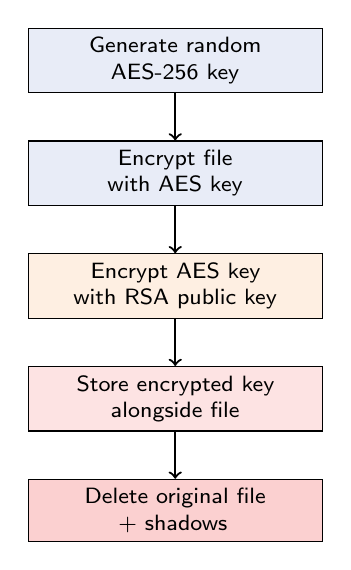
\begin{tikzpicture}[font=\sffamily\footnotesize, node distance=0.6cm]
        \node[rectangle, draw, fill=primaryblue!10, text width=3.5cm, align=center] (gen) {Generate random\\AES-256 key};
        \node[rectangle, draw, fill=primaryblue!10, text width=3.5cm, align=center, below=of gen] (enc) {Encrypt file\\with AES key};
        \node[rectangle, draw, fill=accentorange!15, text width=3.5cm, align=center, below=of enc] (wrap) {Encrypt AES key\\with RSA public key};
        \node[rectangle, draw, fill=accentred!15, text width=3.5cm, align=center, below=of wrap] (store) {Store encrypted key\\alongside file};
        \node[rectangle, draw, fill=accentred!25, text width=3.5cm, align=center, below=of store] (del) {Delete original file\\+ shadows};

        \draw[->, thick] (gen) -- (enc);
        \draw[->, thick] (enc) -- (wrap);
        \draw[->, thick] (wrap) -- (store);
        \draw[->, thick] (store) -- (del);
      \end{tikzpicture}
    \end{column}
  \end{columns}
\end{frame}

% ============================================================
% SECTION 7: DETECTION AND DEFENSE
% ============================================================
\section{Detection and Defense}

\begin{frame}{Detection Approaches}
  \begin{columns}[T]
    \begin{column}{0.48\textwidth}
      \textbf{Static Analysis:}
      \begin{itemize}
        \item \textbf{Signature-based:} Known malware hashes/patterns
        \item \textbf{YARA rules:} Custom pattern matching
        \item \textbf{Heuristic:} Suspicious API imports, strings
        \item \textbf{Limitation:} Easily bypassed by polymorphism
      \end{itemize}

      \vspace{0.5em}
      \textbf{Dynamic/Behavioral Analysis:}
      \begin{itemize}
        \item Sandbox execution (Cuckoo, Any.Run)
        \item API call monitoring
        \item File system activity patterns
        \item Registry modification tracking
        \item Network traffic analysis (C2 beaconing)
      \end{itemize}
    \end{column}
    \begin{column}{0.48\textwidth}
      \textbf{Machine Learning:}
      \begin{itemize}
        \item Anomaly detection on file I/O patterns
        \item Entropy analysis (encrypted files have high entropy)
        \item Process behavior classification
        \item Network traffic anomaly detection
      \end{itemize}

      \vspace{0.5em}
      \textbf{Key Indicators of Ransomware:}
      \begin{itemize}
        \item Rapid file renaming (adding extensions)
        \item Mass file read + write operations
        \item Shadow copy deletion commands
        \item Unusual encryption API usage
        \item Beaconing to unknown IPs/domains
        \item Creation of ransom note files
      \end{itemize}
    \end{column}
  \end{columns}
\end{frame}

\begin{frame}{Prevention: The Defense-in-Depth Approach}
  \begin{columns}[T]
    \begin{column}{0.32\textwidth}
      \begin{block}{Technical Controls}
        \footnotesize
        \begin{itemize}
          \item \textbf{Backups:} 3-2-1 rule (3 copies, 2 media, 1 offsite)
          \item \textbf{Patching:} Automated vulnerability management
          \item \textbf{EDR/XDR:} Real-time behavioral detection
          \item \textbf{Network segmentation}
          \item \textbf{MFA everywhere}
          \item \textbf{Email filtering} (SPF, DKIM, DMARC)
          \item \textbf{Application whitelisting}
        \end{itemize}
      \end{block}
    \end{column}
    \begin{column}{0.32\textwidth}
      \begin{block}{Organizational Controls}
        \footnotesize
        \begin{itemize}
          \item Security awareness training
          \item Phishing simulations
          \item Incident response plan
          \item Regular tabletop exercises
          \item Least privilege access
          \item Vendor risk management
          \item Cyber insurance
        \end{itemize}
      \end{block}
    \end{column}
    \begin{column}{0.32\textwidth}
      \begin{block}{Monitoring \& Response}
        \footnotesize
        \begin{itemize}
          \item 24/7 SOC operations
          \item SIEM log correlation
          \item Threat intelligence feeds
          \item Honeypot / canary files
          \item Automated containment
          \item Forensic readiness
          \item Communication plan
        \end{itemize}
      \end{block}
    \end{column}
  \end{columns}

  \vspace{0.5em}
  \begin{center}
    \textcolor{textgray}{\footnotesize \textbf{No single control is sufficient.} Defense requires layers across people, process, and technology.}
  \end{center}
\end{frame}

\begin{frame}{Incident Response}
  \begin{columns}[T]
    \begin{column}{0.48\textwidth}
      \textbf{Immediate Actions (First 4 Hours):}
      \begin{enumerate}
        \item \alert{Isolate} affected systems from network
        \item Preserve forensic evidence (memory dumps, logs)
        \item Identify ransomware strain (ID Ransomware, No More Ransom)
        \item Assess scope of compromise
        \item Notify CISO, legal, and management
        \item Engage incident response team
      \end{enumerate}

      \vspace{0.5em}
      \begin{dangerbox}{Do NOT}
        \begin{itemize}
          \item Shut down systems (lose memory forensics)
          \item Pay ransom immediately
          \item Communicate via compromised email
          \item Delete ransom notes (contain strain info)
        \end{itemize}
      \end{dangerbox}
    \end{column}
    \begin{column}{0.48\textwidth}
      \textbf{Recovery Steps:}
      \begin{enumerate}
        \item Restore from verified clean backups
        \item Check for free decryptors (No More Ransom project)
        \item Rebuild compromised systems from scratch
        \item Reset ALL credentials (assume full compromise)
        \item Harden environment before reconnecting
        \item Monitor for re-infection (attackers often leave backdoors)
      \end{enumerate}

      \vspace{0.5em}
      \begin{infobox}{To Pay or Not to Pay?}
        \textbf{Recommendation: Do not pay.}\\
        $\bullet$ No guarantee of decryption (8\% never get data back)\\
        $\bullet$ Funds future attacks\\
        $\bullet$ May violate sanctions (OFAC)\\
        $\bullet$ 80\% of payers are attacked again
      \end{infobox}
    \end{column}
  \end{columns}
\end{frame}

% ============================================================
% SECTION 8: LEGAL AND ETHICAL DIMENSIONS
% ============================================================
\section{Legal and Ethical Dimensions}

\begin{frame}{Legal Framework}
  \begin{columns}[T]
    \begin{column}{0.48\textwidth}
      \textbf{For Attackers:}
      \begin{itemize}
        \item \textbf{US:} Computer Fraud and Abuse Act (CFAA) -- up to 20 years
        \item \textbf{EU:} Directive 2013/40/EU on attacks against information systems
        \item \textbf{Germany:} \S 303a/b StGB (data tampering, computer sabotage)
        \item International cooperation via Budapest Convention
        \item OFAC sanctions make payments to certain groups illegal
      \end{itemize}

      \vspace{0.3em}
      \textbf{Notable Prosecutions:}
      \begin{itemize}
        \item REvil: Multiple arrests (Russia, Romania, Ukraine)
        \item NetWalker: Canadian affiliate sentenced to 7 years
        \item Hive: Infrastructure seized by FBI (Jan 2023)
      \end{itemize}
    \end{column}
    \begin{column}{0.48\textwidth}
      \textbf{For Victims:}
      \begin{itemize}
        \item \textbf{GDPR:} Mandatory 72-hour breach notification
        \item Potential fines up to 4\% of annual turnover
        \item SEC reporting requirements (US public companies)
        \item Duty of care to customers and employees
        \item Insurance claim requirements
      \end{itemize}

      \vspace{0.5em}
      \begin{warnbox}{Ethical Research}
        Studying ransomware for defense is essential but must be done:
        \begin{itemize}
          \item In isolated lab environments only
          \item With proper authorization
          \item Following responsible disclosure
          \item Never on production systems
        \end{itemize}
      \end{warnbox}
    \end{column}
  \end{columns}
\end{frame}

% ============================================================
% SECTION 9: FUTURE TRENDS
% ============================================================
\section{Future Trends and Challenges}

\begin{frame}{Emerging Threats}
  \begin{columns}[T]
    \begin{column}{0.48\textwidth}
      \textbf{AI-Powered Ransomware:}
      \begin{itemize}
        \item Automated target selection and vulnerability discovery
        \item AI-generated phishing (indistinguishable from humans)
        \item Adaptive evasion (learning from detection attempts)
        \item Automated negotiation bots
        \item Deepfake-enhanced social engineering
      \end{itemize}

      \vspace{0.5em}
      \textbf{New Attack Surfaces:}
      \begin{itemize}
        \item IoT devices (smart factories, medical devices)
        \item Cloud infrastructure (S3 bucket encryption)
        \item SaaS platforms
        \item Operational Technology (OT/ICS/SCADA)
        \item Autonomous vehicles and smart cities
      \end{itemize}
    \end{column}
    \begin{column}{0.48\textwidth}
      \textbf{Post-Quantum Threat:}
      \begin{itemize}
        \item Quantum computers could break RSA/ECC
        \item ``Harvest now, decrypt later'' concern
        \item NIST post-quantum cryptography standards
        \item Migration timeline: 10--15 years
      \end{itemize}

      \vspace{0.5em}
      \textbf{Geopolitical Dimension:}
      \begin{itemize}
        \item State-sponsored groups (APT) using ransomware as cover
        \item Cyber warfare component (Russia/Ukraine conflict)
        \item Sanctions complicating ransom payments
        \item International cyber norms (UN GGE)
        \item Private sector ``hacking back'' debates
      \end{itemize}

      \vspace{0.3em}
      \begin{infobox}{Research Priorities}
        Zero-day detection, automated IR, post-quantum crypto, cross-border prosecution frameworks.
      \end{infobox}
    \end{column}
  \end{columns}
\end{frame}

% ============================================================
% SECTION 10: CONCLUSION
% ============================================================
\section{Conclusion}

\begin{frame}{Key Takeaways}
  \begin{columns}[T]
    \begin{column}{0.32\textwidth}
      \begin{block}{The Threat}
        \footnotesize
        Ransomware has evolved from simple screen lockers into a \textbf{multi-billion dollar} criminal industry with sophisticated supply chains, professional services, and nation-state involvement.
      \end{block}
    \end{column}
    \begin{column}{0.32\textwidth}
      \begin{block}{The Challenge}
        \footnotesize
        \textbf{No silver bullet} exists. Attackers continuously adapt. The barrier to entry is lower than ever with RaaS models. AI will accelerate both offense and defense.
      \end{block}
    \end{column}
    \begin{column}{0.32\textwidth}
      \begin{block}{The Response}
        \footnotesize
        Defense requires \textbf{layered security}: technical controls, human awareness, tested incident response plans, and international cooperation.
      \end{block}
    \end{column}
  \end{columns}

  \vspace{0.8em}

  \begin{dangerbox}{Final Thought}
    The question is not \textit{if} your organization will face a ransomware attack, but \textit{when}. The difference between a minor incident and a catastrophic event is \textbf{preparation}.
  \end{dangerbox}
\end{frame}

% ============================================================
% REFERENCES
% ============================================================
\begin{frame}{References}
  \begin{thebibliography}{99}
    \setbeamertemplate{bibliography item}[text]
    \bibitem{enisa} ENISA (2024): \textit{Threat Landscape Report 2024}. European Union Agency for Cybersecurity.
    \bibitem{age} Razulla, B. et al.: \textit{The Age of Ransomware: A Survey on the Evolution, Taxonomy, and Research Directions}.
    \bibitem{sophos} Sophos (2024): \textit{The State of Ransomware 2024}. Annual survey report.
    \bibitem{mandiant} Mandiant (2024): \textit{M-Trends 2024}. Special report on cyber threat trends.
    \bibitem{cisa} CISA: \textit{\#StopRansomware Guide}. Joint publication with FBI and NSA.
    \bibitem{mitre} MITRE ATT\&CK: \textit{Enterprise Matrix}. \url{https://attack.mitre.org}
    \bibitem{nomoreransom} No More Ransom Project: \url{https://www.nomoreransom.org}
    \bibitem{oz} Oz, H. et al.: \textit{A Survey on Ransomware: Evolution, Taxonomy, and Defense Solutions}.
  \end{thebibliography}
\end{frame}

\end{document}
